A large number of problems in science and engineering, robotics and game playing, resource management, financial portfolio management, medical treatment design, ad placement, website optimization and packet routing can be modeled as sequential decision-making under uncertainty. Many of these real-world interesting
sequential decision-making problems can be formulated as reinforcement learning (RL) problems (see \citep{bertsekas1996neuro}, \citep{sutton1998reinforcement}). In an RL problem, an agent interacts with a dynamic, stochastic, and unknown environment, with the goal of finding an action-selection strategy or policy that optimizes some long-term performance measure. Every time when the agent interacts with the environment it receives a signal/reward from the environment based on which it modifies its policy. The agent learns to optimize the choice of actions over several time steps which is learned from the sequences of data that it receives from the environment. This is the crux of online sequential learning. 

    This is in contrast to supervised learning methods that deal with labeled data which are independently and identically distributed (i.i.d.) samples from the considered domain and train some classifier on the entire training dataset to learn the pattern of this distribution to predict the labels of future samples (test dataset) with the assumption that it is sampled from the same domain. In contrast to this, an RL agent learns from the samples that are collected from the trajectories generated by its sequential interaction with the system. For an RL agent, the trajectory consists of a series of sequential interactions whereby it transitions from one state to another following some dynamics intrinsic to the environment while collecting the reward till some stopping condition is reached. This is known as an episode. Here, for an action $a_t$ taken by the agent at the $t$-th timestep, the agent transitions from its current state denoted by $S_{t}$ to state $S_{t+1}$ and observes the reward $R(s_t,a_t)$. An illustrative image depicting the reinforcement learning scenario is shown in Figure \ref{fig:rl}.
    

\begin{figure}[!th]
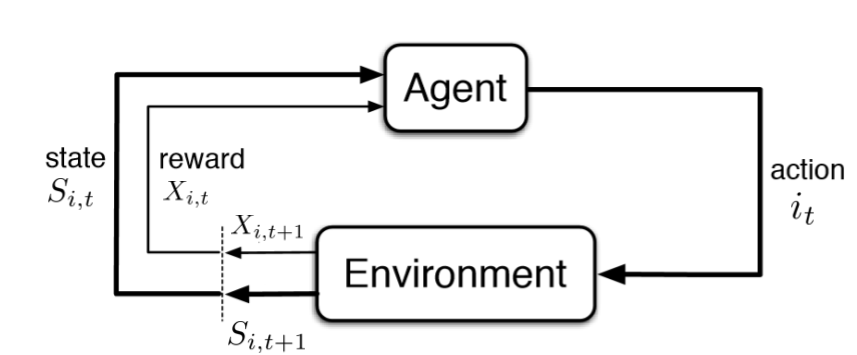
\includegraphics[scale=0.4]{img/RL1.png}
\caption{Reinforcement Learning}
\label{fig:rl}
\end{figure}

In the healthcare domain, there exists many scenarios in which the treatment involves taking a series of decisions over a long time. After every medical decision is made, and a treatment administered the condition of the patient changes. Based on this new condition of the patient medical practitioners may alter their evaluation policy to administer a new set of treatments or may continue with the last policy with the same dosage. Notice, that this is quite similar to the general RL framework where the condition of the patient can be defined by the state $S_t$, the treatment administered can be defined by action $a_t$ and after administering the treatment the new condition that the patient transitions to can be defined by $S_{t+1}$. We will formalize this setting in Section \ref{review:mdp} while we will illustrate several challenges where this simple framework will fail in real world scenarios in Section \ref{review:complexity}.

	As mentioned in \citet{DBLP:conf/embc/NematiGC16} RL is particularly well-suited for the medication dosing problem given the sequential nature of clinical treatment where multiple treatment decision are performed without immediate knowledge of effectiveness. Indeed, the lack of a one-to-one correspondence between actions and outcomes makes it difficult to assign credit or blame to individual actions along the way to an intermediate or terminal outcome. Moreover, the effect of interventions for a given patient can be non-deterministic, and attempting to predict the effects of a series of treatments over time only causes more uncertainty.

